% A concrete visual account of the joint demodulation and decoding problem
% (CX-62--CX-67).  The numerical example is generated by
% joint_tutorial_worked_example.py.  Receiver actions follow Algorithms 1--5
% of juna_joint_ieee.tex.
\documentclass[aspectratio=169,10pt]{beamer}
\usepackage[T1]{fontenc}
\usepackage{amsmath,amssymb,amsfonts}
\usepackage{bm}
\usepackage{tikz}
\usepackage{xcolor}
\usetikzlibrary{arrows.meta,positioning,shapes,calc}

\definecolor{parchment}{HTML}{F4E8C8}
\definecolor{paper}{HTML}{FAF1D8}
\definecolor{ink}{HTML}{1A1A1A}
\definecolor{inkgray}{HTML}{5A5A5A}
\definecolor{accentred}{HTML}{8B1A1A}
\definecolor{accentgreen}{HTML}{2D5F2C}
\definecolor{accentblue}{HTML}{1F4E79}
\definecolor{redbg}{HTML}{F7E0DE}
\definecolor{grnbg}{HTML}{E0EBDC}
\definecolor{blubg}{HTML}{DDE6EF}
\definecolor{labelbg}{HTML}{EFE0B0}

\usefonttheme{serif}
\setbeamercolor{background canvas}{bg=parchment}
\setbeamercolor{normal text}{fg=ink}
\setbeamercolor{structure}{fg=ink}
\setbeamercolor{frametitle}{fg=ink,bg=parchment}
\setbeamercolor{title}{fg=ink}
\setbeamercolor{itemize item}{fg=ink}
\setbeamercolor{itemize subitem}{fg=ink}
\setbeamercolor{item}{fg=ink}
\setbeamercolor{caption name}{fg=ink}
\setbeamertemplate{navigation symbols}{}
\setbeamertemplate{itemize item}{\textbullet}

\setbeamertemplate{frametitle}{%
  \vspace{0.30em}%
  \begin{center}%
    {\bfseries\Large\insertframetitle\par}%
    \vspace{0.28em}%
    {\color{ink}\rule{0.86\paperwidth}{0.4pt}}%
  \end{center}%
  \vspace{0.10em}%
}
\setbeamertemplate{footline}{%
  \hbox to \paperwidth{\hfil\itshape\small\insertframenumber\hspace{0.7em}}%
  \vspace{0.35em}%
}

\newcommand{\vY}{\bm{Y}}
\newcommand{\vy}{\bm{y}}
\newcommand{\vA}{\bm{A}}
\newcommand{\vB}{\bm{B}}
\newcommand{\valpha}{\bm{\alpha}}
\newcommand{\vn}{\bm{n}}
\newcommand{\vs}{\bm{s}}
\newcommand{\vW}{\bm{W}}
\newcommand{\T}{^{\mathsf T}}
\newcommand{\Hh}{^{\mathsf H}}
\newcommand{\norm}[1]{\left\lVert #1\right\rVert}
\DeclareMathOperator*{\argmin}{arg\,min}

\tikzset{
  flowbox/.style={draw=ink,fill=paper,line width=0.6pt,
                  minimum width=2.5cm,minimum height=1.0cm,
                  align=center,font=\small\bfseries,inner sep=4pt},
  smallbox/.style={draw=ink,fill=paper,line width=0.4pt,
                   minimum width=0.7cm,minimum height=0.55cm,
                   inner sep=2pt,align=center,font=\footnotesize\itshape},
  method/.style={draw=accentgreen,fill=grnbg,line width=1.0pt,
                 align=center,font=\small\bfseries,inner sep=6pt},
  issue/.style={draw=accentred,fill=redbg,line width=1.0pt,
                align=center,font=\small\bfseries,inner sep=6pt},
  idea/.style={draw=accentblue,fill=blubg,line width=1.0pt,
               align=center,font=\small\bfseries,inner sep=6pt},
  flowarr/.style={-{Stealth[length=2.5mm,width=2mm]},line width=0.7pt},
  softarr/.style={-{Stealth[length=2mm,width=1.6mm]},line width=0.5pt,color=inkgray}
}

\newcommand{\bottomnote}[1]{%
  \begin{center}{\itshape\small #1}\end{center}}

\newcommand{\papercover}[4]{%
  \begin{frame}[plain]
    \vfill
    \begin{center}
      {\bfseries\Huge #1\par}
      \vspace{0.8cm}
      {\Large #2\par}
      \vspace{0.35cm}
      {\itshape\large\color{inkgray}#3\par}
      \vspace{0.55cm}
      {\small\texttt{\detokenize{#4}}\par}
    \end{center}
    \vfill
  \end{frame}}

\newcommand{\twocolmodel}[4]{%
  \begin{columns}[T,onlytextwidth]
    \begin{column}{0.48\textwidth}#1\end{column}
    \begin{column}{0.48\textwidth}#2\end{column}
  \end{columns}
  \bottomnote{#3\\#4}}


\usetikzlibrary{fit,decorations.pathreplacing}

\newcommand{\Kset}{\mathcal K}
\newcommand{\Bset}{\mathcal B}
\newcommand{\Pset}{\mathcal P}
\newcommand{\E}{\mathbb E}

\tikzset{
  card/.style={draw=ink,fill=paper,line width=0.55pt,rounded corners=2pt,
               align=center,inner sep=5pt,font=\small},
  goodcard/.style={draw=accentgreen,fill=grnbg,line width=0.85pt,
                   rounded corners=2pt,align=center,inner sep=5pt,font=\small},
  badcard/.style={draw=accentred,fill=redbg,line width=0.85pt,
                  rounded corners=2pt,align=center,inner sep=5pt,font=\small},
  bluecard/.style={draw=accentblue,fill=blubg,line width=0.85pt,
                   rounded corners=2pt,align=center,inner sep=5pt,font=\small},
  panel/.style={draw=ink,fill=parchment,line width=0.9pt,rounded corners=3pt},
  redarr/.style={-{Stealth[length=2.5mm,width=2mm]},line width=0.85pt,
                  draw=accentred},
  greenarr/.style={-{Stealth[length=2.5mm,width=2mm]},line width=0.85pt,
                    draw=accentgreen},
  bluearr/.style={-{Stealth[length=2.5mm,width=2mm]},line width=0.85pt,
                   draw=accentblue},
  grayarr/.style={-{Stealth[length=2.2mm,width=1.8mm]},line width=0.65pt,
                   draw=inkgray},
  cpbrace/.style={decorate,decoration={brace,amplitude=5pt,raise=2pt},
                  line width=0.6pt,color=inkgray},
  bit/.style={circle,draw=accentblue,fill=blubg,line width=0.7pt,
              minimum size=7mm,font=\scriptsize},
  check/.style={circle,draw=accentred,fill=redbg,line width=0.8pt,
                minimum size=8mm,font=\scriptsize\bfseries}
}

\begin{document}

% =====================================================================
% 1. Cover
% =====================================================================
\begin{frame}[plain]
  \centering
  \vspace{0.18cm}
  {\small\color{inkgray}\texttt{juna\_joint\_ieee.tex}, in pictures\par}
  \vspace{0.14cm}
  {\bfseries\Huge The Joint Demodulation and Decoding Problem\par}
  \vspace{0.12cm}
  {\Large Carrier 4 inside the frame-wide receiver\par}
  \vspace{0.40cm}

  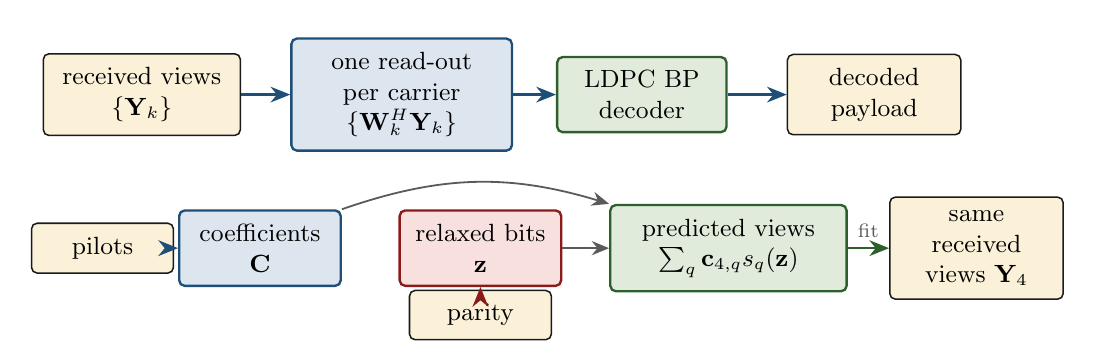
\begin{tikzpicture}[x=1cm,y=1cm]
    \path[use as bounding box] (-6.7,-2.0) rectangle (6.7,1.8);

    \node[card,text width=2.15cm] (views) at (-5.25,0.95)
      {received views\\$\{\mathbf Y_k\}$};
    \node[bluecard,text width=2.45cm] (readout) at (-1.95,0.95)
      {one read-out per carrier\\$\{\mathbf W_k^H\mathbf Y_k\}$};
    \node[goodcard,text width=1.80cm] (bp) at (1.10,0.95)
      {LDPC BP\\decoder};
    \node[card,text width=1.85cm] (payload) at (4.05,0.95)
      {decoded\\payload};
    \draw[bluearr] (views) -- (readout);
    \draw[bluearr] (readout) -- (bp);
    \draw[bluearr] (bp) -- (payload);

    \node[bluecard,text width=1.70cm] (coef) at (-3.75,-1.00)
      {coefficients\\$\mathbf C$};
    \node[badcard,text width=1.70cm] (bits) at (-0.95,-1.00)
      {relaxed bits\\$\mathbf z$};
    \node[goodcard,text width=2.65cm] (pred) at (2.20,-1.00)
      {predicted views\\$\sum_q\mathbf c_{4,q}s_q(\mathbf z)$};
    \node[card,text width=1.85cm] (sameviews) at (5.35,-1.00)
      {same received\\views $\mathbf Y_4$};
    \node[card,text width=1.45cm] (pilots) at (-5.75,-1.00) {pilots};
    \node[card,text width=1.45cm] (parity) at (-0.95,-1.85) {parity};
    \draw[bluearr] (pilots) -- (coef);
    \draw[redarr] (parity) -- (bits);
    \draw[grayarr] (coef.north east) to[bend left=18] (pred.north west);
    \draw[grayarr] (bits) -- (pred);
    \draw[greenarr] (pred) -- (sameviews)
      node[midway,above,font=\scriptsize,color=inkgray] {fit};
  \end{tikzpicture}

  \vspace{0.12cm}
  {\small\color{inkgray}The combiner is a read-out.  The joint problem
   scores the coefficients and relaxed bits against the received views.\par}
\end{frame}

% =====================================================================
% 2. The read-out
% =====================================================================
\begin{frame}{The read-out}
  \centering
  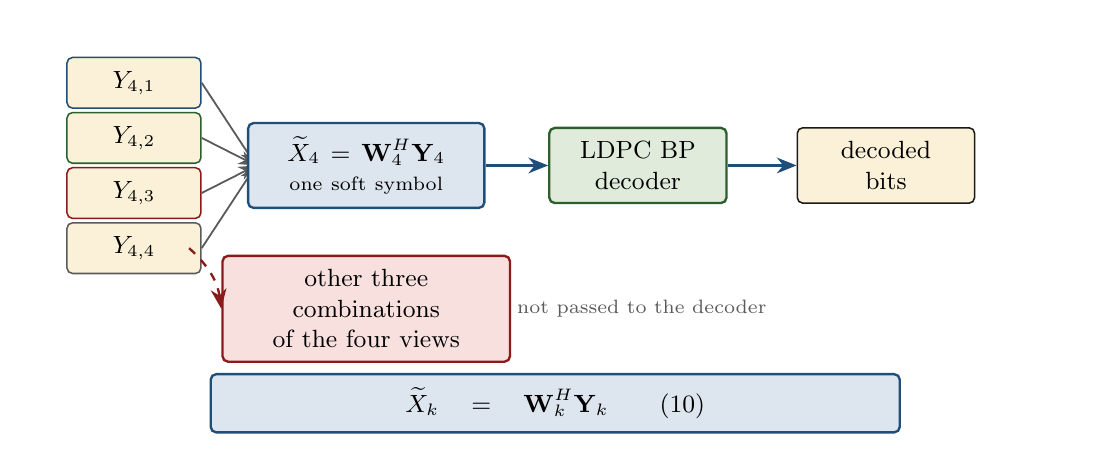
\begin{tikzpicture}[x=1cm,y=1cm]
    \path[use as bounding box] (-6.7,-2.75) rectangle (6.7,2.35);

    \foreach \m/\yy/\col in {1/1.65/accentblue,2/0.95/accentgreen,
                             3/0.25/accentred,4/-0.45/inkgray}{
      \node[card,draw=\col,text width=1.35cm] (y\m) at (-5.35,\yy)
        {$Y_{4,\m}$};
      \draw[grayarr] (y\m.east) -- (-3.80,0.60);
    }
    \node[bluecard,text width=2.65cm] (combine) at (-2.40,0.60)
      {$\widetilde X_4=\mathbf W_4^H\mathbf Y_4$\\[-0.05em]
       \scriptsize one soft symbol};
    \node[goodcard,text width=1.90cm] (bp) at (1.05,0.60)
      {LDPC BP\\decoder};
    \node[card,text width=1.90cm] (bits) at (4.20,0.60)
      {decoded\\bits};
    \draw[bluearr] (combine) -- (bp);
    \draw[bluearr] (bp) -- (bits);

    \node[badcard,text width=3.30cm] (other) at (-2.40,-1.22)
      {other three combinations\\of the four views};
    \draw[redarr,dashed] (-4.65,-0.45) to[bend left=20] (other.west);
    \node[font=\scriptsize,color=inkgray] at (1.10,-1.22)
      {not passed to the decoder};

    \node[bluecard,text width=8.40cm] at (0,-2.42)
      {\(\displaystyle
        \widetilde X_k=\mathbf W_k^H\mathbf Y_k
        \qquad\text{(10)}\)};
  \end{tikzpicture}
  \bottomnote{The read-out keeps one combination of a carrier's views for the decoder.  Here \(\mathbf Y_k\) contains the \(M\) views and \(\mathbf W_k\) contains one weight per view.}
\end{frame}

% =====================================================================
% 3. Scalar or vector?
% =====================================================================
\begin{frame}{Scalar or vector?}
  \centering
  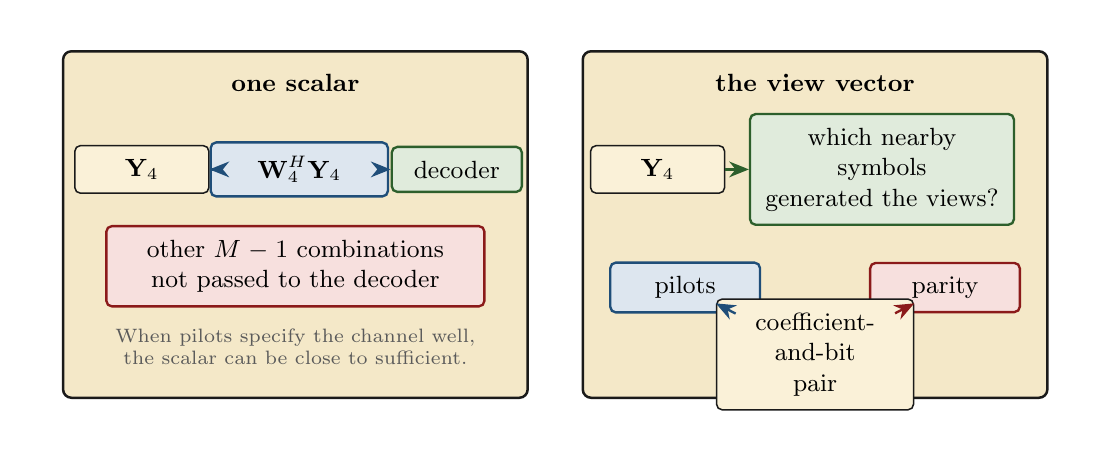
\begin{tikzpicture}[x=1cm,y=1cm]
    \path[use as bounding box] (-6.7,-2.75) rectangle (6.7,2.35);

    \draw[panel] (-6.25,-2.35) rectangle (-0.35,2.05);
    \node[font=\small\bfseries] at (-3.30,1.65) {one scalar};
    \node[card,text width=1.35cm] (ys) at (-5.25,0.55) {$\mathbf Y_4$};
    \node[bluecard,text width=1.90cm] (ws) at (-3.25,0.55)
      {$\mathbf W_4^H\mathbf Y_4$};
    \node[goodcard,text width=1.30cm] (ds) at (-1.25,0.55) {decoder};
    \draw[bluearr] (ys) -- (ws);
    \draw[bluearr] (ws) -- (ds);
    \node[badcard,text width=4.45cm] at (-3.30,-0.68)
      {other \(M-1\) combinations\\not passed to the decoder};
    \node[font=\scriptsize,color=inkgray,text width=4.9cm,align=center]
      at (-3.30,-1.70)
      {When pilots specify the channel well, the scalar can be close to
       sufficient.};

    \draw[panel] (0.35,-2.35) rectangle (6.25,2.05);
    \node[font=\small\bfseries] at (3.30,1.65) {the view vector};
    \node[card,text width=1.35cm] (yv) at (1.30,0.55) {$\mathbf Y_4$};
    \node[goodcard,text width=3.00cm] (ask) at (4.15,0.55)
      {which nearby symbols\\generated the views?};
    \draw[greenarr] (yv) -- (ask);
    \node[bluecard,text width=1.55cm] (p) at (1.65,-0.95) {pilots};
    \node[badcard,text width=1.55cm] (r) at (4.95,-0.95) {parity};
    \node[card,text width=2.15cm] (cz) at (3.30,-1.80)
      {coefficient-and-bit\\pair};
    \draw[bluearr] (p) -- (cz);
    \draw[redarr] (r) -- (cz);
  \end{tikzpicture}
  \bottomnote{The joint search retains the view vector, uses pilots to constrain the coefficients, and uses parity checks to restrict the coded bits.}
\end{frame}

% =====================================================================
% 4. A worked example
% =====================================================================
\begin{frame}{A worked example}
  \centering
  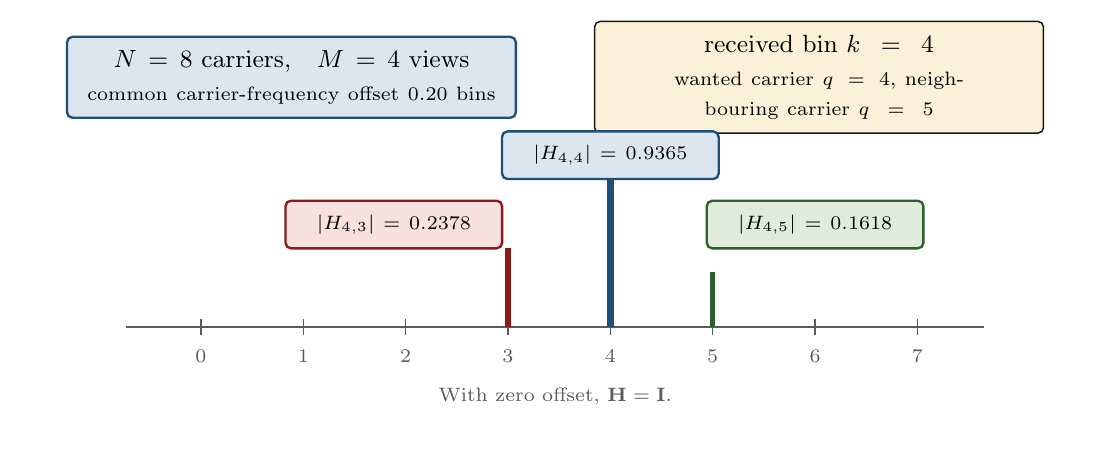
\begin{tikzpicture}[x=1cm,y=1cm]
    \path[use as bounding box] (-6.7,-2.75) rectangle (6.7,2.35);

    \node[bluecard,text width=5.35cm] at (-3.35,1.72)
      {\(N=8\) carriers,\quad \(M=4\) views\\[0.08em]
       \scriptsize common carrier-frequency offset \(0.20\) bins};
    \node[card,text width=5.35cm] at (3.35,1.72)
      {received bin \(k=4\)\\[0.08em]
       \scriptsize wanted carrier \(q=4\), neighbouring carrier \(q=5\)};

    \draw[line width=0.6pt,color=inkgray] (-5.45,-1.45) -- (5.45,-1.45);
    \foreach \x/\lab in {-4.5/0,-3.2/1,-1.9/2,-0.6/3,0.7/4,2.0/5,3.3/6,4.6/7}{
      \draw[line width=0.5pt,color=inkgray] (\x,-1.55) -- (\x,-1.35);
      \node[font=\scriptsize,color=inkgray] at (\x,-1.82) {\lab};
    }
    \draw[line width=2.0pt,color=accentred] (-0.6,-1.45) -- (-0.6,-0.45);
    \draw[line width=2.5pt,color=accentblue] (0.7,-1.45) -- (0.7,0.55);
    \draw[line width=2.0pt,color=accentgreen] (2.0,-1.45) -- (2.0,-0.75);
    \node[badcard,text width=2.40cm,font=\scriptsize] at (-2.05,-0.15)
      {\(\left|H_{4,3}\right|=0.2378\)};
    \node[bluecard,text width=2.40cm,font=\scriptsize] at (0.70,0.73)
      {\(\left|H_{4,4}\right|=0.9365\)};
    \node[goodcard,text width=2.40cm,font=\scriptsize] at (3.30,-0.15)
      {\(\left|H_{4,5}\right|=0.1618\)};
    \node[font=\scriptsize,color=inkgray] at (0,-2.33)
      {With zero offset, \(\mathbf H=\mathbf I\).};
  \end{tikzpicture}
  \bottomnote{The following pages keep carrier \(4\), its four views, and neighbouring carrier \(5\) visible.  This is a toy calculation, not a measured Red channel.}
\end{frame}

% =====================================================================
% 5. Four views
% =====================================================================
\begin{frame}{Four views}
  \centering
  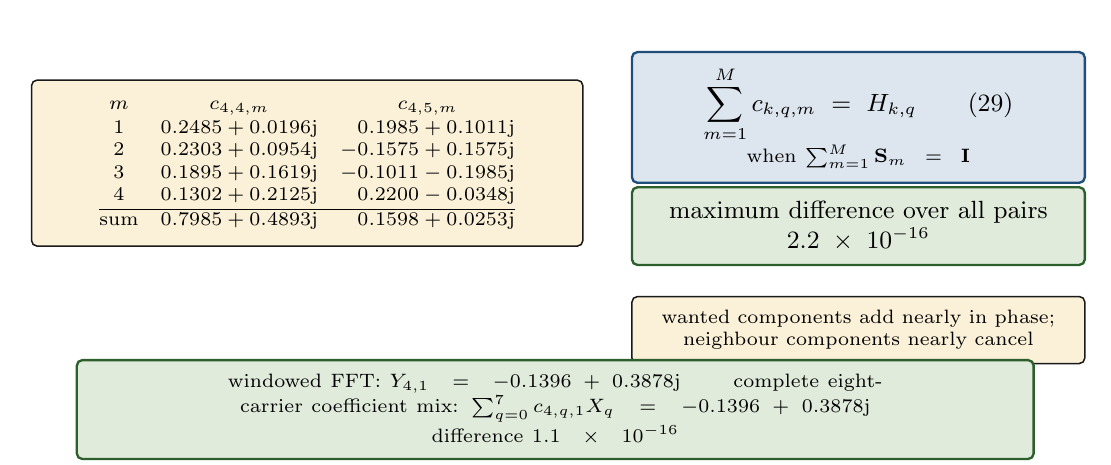
\begin{tikzpicture}[x=1cm,y=1cm]
    \path[use as bounding box] (-6.7,-2.78) rectangle (6.7,2.42);

    \node[card,text width=6.65cm] at (-3.15,0.70)
      {\scriptsize
       \begin{tabular}{@{}c@{\quad}c@{\quad}c@{}}
       \(m\) & \(c_{4,4,m}\) & \(c_{4,5,m}\)\\[0.10em]
       1 & \(0.2485+0.0196\mathrm j\) & \(\phantom{-}0.1985+0.1011\mathrm j\)\\
       2 & \(0.2303+0.0954\mathrm j\) & \(-0.1575+0.1575\mathrm j\)\\
       3 & \(0.1895+0.1619\mathrm j\) & \(-0.1011-0.1985\mathrm j\)\\
       4 & \(0.1302+0.2125\mathrm j\) & \(\phantom{-}0.2200-0.0348\mathrm j\)\\[0.10em]
       \hline
       sum & \(0.7985+0.4893\mathrm j\) & \(\phantom{-}0.1598+0.0253\mathrm j\)
       \end{tabular}};

    \node[bluecard,text width=5.40cm] at (3.85,1.28)
      {\(\displaystyle
       \sum_{m=1}^{M}c_{k,q,m}=H_{k,q}\qquad\text{(29)}\)\\[-0.02em]
       \scriptsize when \(\sum_{m=1}^{M}\mathbf S_m=\mathbf I\)};
    \node[goodcard,text width=5.40cm] at (3.85,-0.10)
      {maximum difference over all pairs\\
       \(2.2\times10^{-16}\)};
    \node[card,text width=5.40cm,font=\scriptsize] at (3.85,-1.42)
      {wanted components add nearly in phase;\\
       neighbour components nearly cancel};

    \node[goodcard,text width=11.80cm] at (0,-2.43)
      {\scriptsize
       windowed FFT: \(Y_{4,1}=-0.1396+0.3878\mathrm j\)
       \qquad complete eight-carrier coefficient mix:
       \(\sum_{q=0}^{7}c_{4,q,1}X_q=-0.1396+0.3878\mathrm j\)\\[-0.02em]
       difference \(1.1\times10^{-16}\)};
  \end{tikzpicture}
  \bottomnote{Each coefficient is one time-local part of the same channel coefficient.  The receiver retains nearby pairs in equation (28); omitted pairs are not asserted to be physically zero.}
\end{frame}

% =====================================================================
% 6. Pilots
% =====================================================================
\begin{frame}{Pilots}
  \centering
  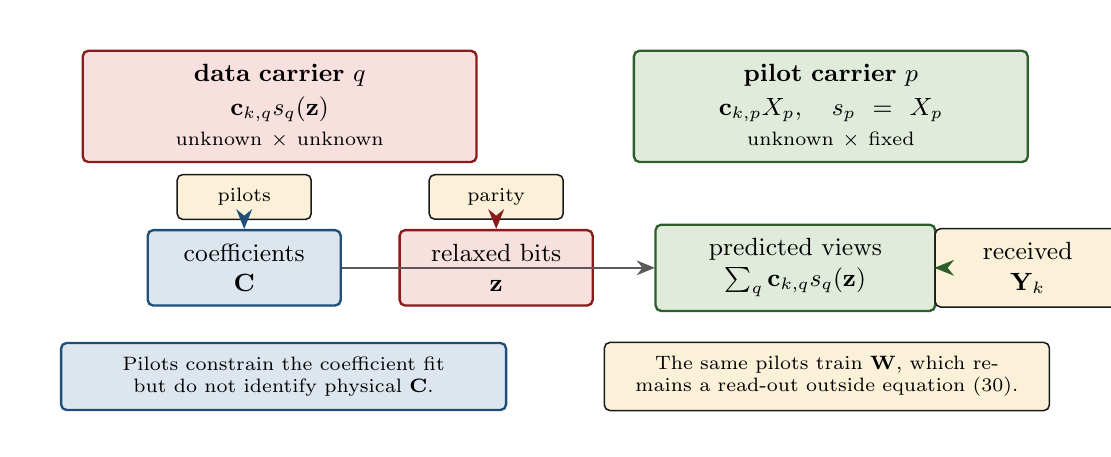
\begin{tikzpicture}[x=1cm,y=1cm]
    \path[use as bounding box] (-6.7,-2.75) rectangle (6.7,2.35);

    \node[badcard,text width=4.65cm] (data) at (-3.50,1.35)
      {\textbf{data carrier \(q\)}\\[0.12em]
       \(\mathbf c_{k,q}s_q(\mathbf z)\)\\
       \scriptsize unknown \(\times\) unknown};
    \node[goodcard,text width=4.65cm] (pilot) at (3.50,1.35)
      {\textbf{pilot carrier \(p\)}\\[0.12em]
       \(\mathbf c_{k,p}X_p,\quad s_p=X_p\)\\
       \scriptsize unknown \(\times\) fixed};

    \node[card,text width=1.35cm,font=\scriptsize] (pnode) at (-3.95,0.20)
      {pilots};
    \node[card,text width=1.35cm,font=\scriptsize] (rnode) at (-0.75,0.20)
      {parity};
    \node[bluecard,text width=2.10cm] (coef) at (-3.95,-0.70)
      {coefficients\\$\mathbf C$};
    \node[badcard,text width=2.10cm] (bits) at (-0.75,-0.70)
      {relaxed bits\\$\mathbf z$};
    \node[goodcard,text width=3.20cm] (model) at (3.05,-0.70)
      {predicted views\\
       \(\sum_q\mathbf c_{k,q}s_q(\mathbf z)\)};
    \node[card,text width=2.00cm] (views) at (6.00,-0.70)
      {received\\$\mathbf Y_k$};
    \draw[bluearr] (pnode) -- (coef);
    \draw[redarr] (rnode) -- (bits);
    \draw[grayarr] (coef) -- (model);
    \draw[grayarr] (bits) -- (model);
    \draw[greenarr] (model) -- (views);

    \node[bluecard,text width=5.30cm,font=\scriptsize] at (-3.45,-2.08)
      {Pilots constrain the coefficient fit but do not identify physical
       \(\mathbf C\).};
    \node[card,text width=5.30cm,font=\scriptsize] at (3.45,-2.08)
      {The same pilots train \(\mathbf W\), which remains a read-out outside
       equation (30).};
  \end{tikzpicture}
  \bottomnote{Pilots constrain the coefficients, while parity checks restrict the coded bits.  Both affect the predicted views through different variables.}
\end{frame}

% =====================================================================
% 7. Relaxed symbol
% =====================================================================
\begin{frame}{Relaxed symbol}
  \centering
  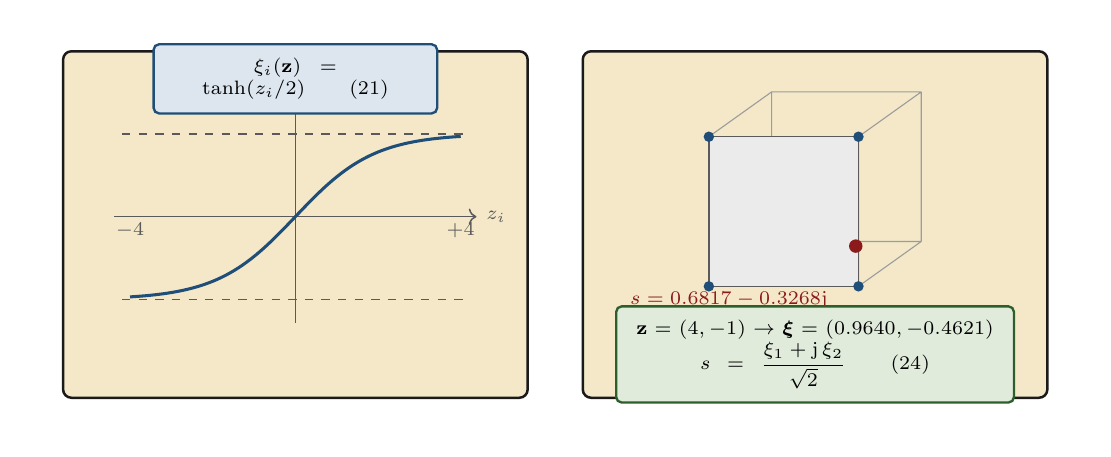
\begin{tikzpicture}[x=1cm,y=1cm]
    \path[use as bounding box] (-6.7,-2.75) rectangle (6.7,2.35);

    \draw[panel] (-6.25,-2.35) rectangle (-0.35,2.05);
    \begin{scope}[shift={(-3.30,-0.05)}]
      \draw[->,line width=0.55pt,color=inkgray] (-2.30,0) -- (2.30,0)
        node[right,font=\scriptsize] {$z_i$};
      \draw[->,line width=0.55pt,color=inkgray] (0,-1.35) -- (0,1.55)
        node[above,font=\scriptsize] {$\xi_i$};
      \draw[dashed,color=inkgray] (-2.20,1.05) -- (2.20,1.05);
      \draw[dashed,color=inkgray] (-2.20,-1.05) -- (2.20,-1.05);
      \draw[line width=1.1pt,color=accentblue,smooth,samples=81,
            domain=-4.20:4.20]
        plot ({0.50*\x},{1.05*tanh(\x/2)});
      \node[bluecard,text width=3.25cm,font=\scriptsize] at (0,1.75)
        {\(\xi_i(\mathbf z)=\tanh(z_i/2)\qquad\text{(21)}\)};
      \node[font=\scriptsize,color=inkgray] at (-2.10,-0.18) {\(-4\)};
      \node[font=\scriptsize,color=inkgray] at (2.10,-0.18) {\(+4\)};
    \end{scope}

    \draw[panel] (0.35,-2.35) rectangle (6.25,2.05);
    \begin{scope}[shift={(3.30,0.30)},scale=0.95]
      \draw[line width=0.4pt,color=inkgray!60]
        (1.42,1.30) -- (-0.58,1.30)
        (0.58,0.70) -- (-1.42,0.70)
        (1.42,-0.70) -- (-0.58,-0.70)
        (0.58,-1.30) -- (-1.42,-1.30)
        (1.42,1.30) -- (1.42,-0.70)
        (0.58,0.70) -- (0.58,-1.30)
        (-0.58,1.30) -- (-0.58,-0.70)
        (-1.42,0.70) -- (-1.42,-1.30)
        (1.42,1.30) -- (0.58,0.70)
        (1.42,-0.70) -- (0.58,-1.30)
        (-0.58,1.30) -- (-1.42,0.70)
        (-0.58,-0.70) -- (-1.42,-1.30);
      \fill[inkgray!12] (0.58,0.70) -- (0.58,-1.30) -- (-1.42,-1.30)
        -- (-1.42,0.70) -- cycle;
      \draw[line width=0.5pt,color=inkgray] (0.58,0.70) -- (0.58,-1.30)
        -- (-1.42,-1.30) -- (-1.42,0.70) -- cycle;
      \foreach \px/\py in {0.58/0.70,0.58/-1.30,-1.42/0.70,-1.42/-1.30}{
        \fill[accentblue] (\px,\py) circle (0.07);
      }
      \fill[accentred] (0.5440,-0.7621) circle (0.09);
      \node[font=\scriptsize,color=accentred,anchor=east] at (0.30,-1.48)
        {$s=0.6817-0.3268\mathrm j$};
    \end{scope}
    \node[goodcard,text width=4.70cm,font=\scriptsize] at (3.30,-1.80)
      {\(\mathbf z=(4,-1)\rightarrow
        \boldsymbol\xi=(0.9640,-0.4621)\)\\
       \(\displaystyle
        s=\frac{\xi_1+\mathrm j\,\xi_2}{\sqrt2}\qquad\text{(24)}\)};
  \end{tikzpicture}
  \bottomnote{Hard bits give the four quadrature phase-shift keying points.  Relaxed bits move the symbol inside the square and provide a differentiable path.  The square is one face of the cube the coded bits span.}
\end{frame}

% =====================================================================
% 8. Parity penalty
% =====================================================================
\begin{frame}{Parity penalty}
  \centering
  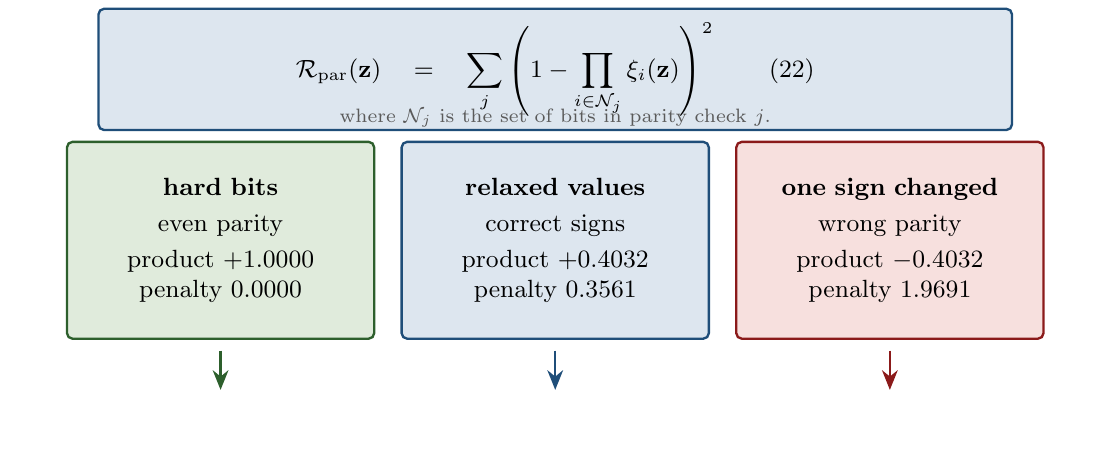
\begin{tikzpicture}[x=1cm,y=1cm]
    \path[use as bounding box] (-6.7,-2.75) rectangle (6.7,2.35);

    \node[bluecard,text width=11.25cm] at (0,1.82)
      {\(\displaystyle
       \mathcal R_{\mathrm{par}}(\mathbf z)=
       \sum_j\left(1-\prod_{i\in\mathcal N_j}
       \xi_i(\mathbf z)\right)^2
       \qquad\text{(22)}\)};
    \node[font=\scriptsize,color=inkgray] at (0,1.20)
      {where \(\mathcal N_j\) is the set of bits in parity check \(j\).};

    \node[goodcard,text width=3.55cm,minimum height=2.50cm] at (-4.25,-0.35)
      {\textbf{hard bits}\\[0.22em]
       even parity\\[0.20em]
       product \(+1.0000\)\\
       penalty \(0.0000\)};
    \node[bluecard,text width=3.55cm,minimum height=2.50cm] at (0,-0.35)
      {\textbf{relaxed values}\\[0.22em]
       correct signs\\[0.20em]
       product \(+0.4032\)\\
       penalty \(0.3561\)};
    \node[badcard,text width=3.55cm,minimum height=2.50cm] at (4.25,-0.35)
      {\textbf{one sign changed}\\[0.22em]
       wrong parity\\[0.20em]
       product \(-0.4032\)\\
       penalty \(1.9691\)};

    \draw[greenarr] (-4.25,-1.75) -- (-4.25,-2.25);
    \draw[bluearr] (0,-1.75) -- (0,-2.25);
    \draw[redarr] (4.25,-1.75) -- (4.25,-2.25);
  \end{tikzpicture}
  \bottomnote{The penalty vanishes on codewords.  Relaxed values with the correct signs remain costly until their magnitudes approach one.}
\end{frame}

% =====================================================================
% 9. One objective
% =====================================================================
\begin{frame}{One objective}
  \centering
  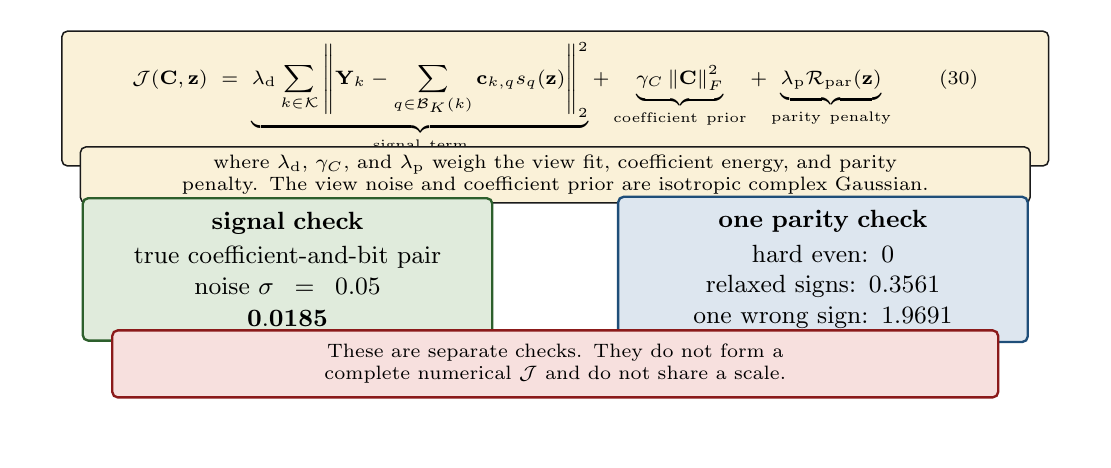
\begin{tikzpicture}[x=1cm,y=1cm]
    \path[use as bounding box] (-6.7,-2.82) rectangle (6.7,2.42);

    \node[card,text width=12.25cm,inner sep=4pt] at (0,1.52)
      {\scriptsize
       \(\displaystyle
       \mathcal J(\mathbf C,\mathbf z)
       =
       \underbrace{\lambda_{\mathrm d}\sum_{k\in\Kset}
       \left\|\mathbf Y_k-\sum_{q\in\Bset_K(k)}
       \mathbf c_{k,q}s_q(\mathbf z)\right\|_2^2}_{\text{signal term}}
       +
       \underbrace{\gamma_C\norm{\mathbf C}_F^2}_{\text{coefficient prior}}
       +
       \underbrace{\lambda_{\mathrm p}
       \mathcal R_{\mathrm{par}}(\mathbf z)}_{\text{parity penalty}}
       \qquad\text{(30)}\)};
    \node[card,text width=11.85cm,font=\scriptsize,inner sep=3pt]
      at (0,0.55)
      {where \(\lambda_{\mathrm d}\), \(\gamma_C\), and
       \(\lambda_{\mathrm p}\) weigh the view fit, coefficient energy, and
       parity penalty.  The view noise and coefficient prior are isotropic
       complex Gaussian.};

    \node[goodcard,text width=4.85cm,minimum height=1.25cm] at (-3.40,-0.65)
      {\textbf{signal check}\\[0.16em]
       true coefficient-and-bit pair\\
       noise \(\sigma=0.05\)\\[0.08em]
       \(\mathbf{0.0185}\)};
    \node[bluecard,text width=4.85cm,minimum height=1.25cm] at (3.40,-0.65)
      {\textbf{one parity check}\\[0.16em]
       hard even: \(0\)\\
       relaxed signs: \(0.3561\)\\
       one wrong sign: \(1.9691\)};

    \node[badcard,text width=10.90cm,font=\scriptsize] at (0,-1.85)
      {These are separate checks.  They do not form a complete numerical
       \(\mathcal J\) and do not share a scale.};
  \end{tikzpicture}
  \bottomnote{Equation (30) scores \(\mathbf C\) and \(\mathbf z\) against the received views.  The combiner \(\mathbf W\) remains outside the objective.}
\end{frame}

% =====================================================================
% 9b. The ring
% =====================================================================
\begin{frame}{The ring}
  \centering
  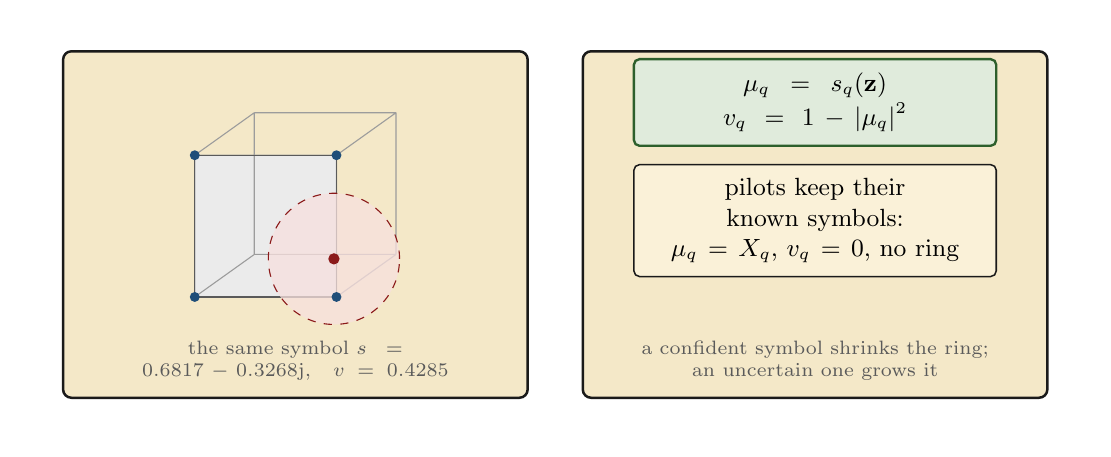
\begin{tikzpicture}[x=1cm,y=1cm]
    \path[use as bounding box] (-6.7,-2.75) rectangle (6.7,2.35);

    \draw[panel] (-6.25,-2.35) rectangle (-0.35,2.05);
    \begin{scope}[shift={(-3.30,0.10)},scale=0.9]
      \fill[inkgray!12] (0.58,0.70) -- (0.58,-1.30) -- (-1.42,-1.30)
        -- (-1.42,0.70) -- cycle;
      \draw[line width=0.4pt,color=inkgray!60]
        (1.42,1.30) -- (-0.58,1.30)
        (0.58,0.70) -- (-1.42,0.70)
        (1.42,-0.70) -- (-0.58,-0.70)
        (0.58,-1.30) -- (-1.42,-1.30)
        (1.42,1.30) -- (1.42,-0.70)
        (0.58,0.70) -- (0.58,-1.30)
        (-0.58,1.30) -- (-0.58,-0.70)
        (-1.42,0.70) -- (-1.42,-1.30)
        (1.42,1.30) -- (0.58,0.70)
        (1.42,-0.70) -- (0.58,-1.30)
        (-0.58,1.30) -- (-1.42,0.70)
        (-0.58,-0.70) -- (-1.42,-1.30);
      \draw[line width=0.5pt,color=inkgray] (0.58,0.70) -- (0.58,-1.30)
        -- (-1.42,-1.30) -- (-1.42,0.70) -- cycle;
      \fill[redbg,opacity=0.75] (0.5440,-0.7621) circle (0.9257);
      \draw[dashed,color=accentred] (0.5440,-0.7621) circle (0.9257);
      \foreach \px/\py in {0.58/0.70,0.58/-1.30,-1.42/0.70,-1.42/-1.30}{
        \fill[accentblue] (\px,\py) circle (0.07);
      }
      \fill[accentred] (0.5440,-0.7621) circle (0.08);
    \end{scope}
    \node[font=\scriptsize,color=inkgray,text width=5.0cm,align=center]
      at (-3.30,-1.88)
      {the same symbol \(s=0.6817-0.3268\mathrm j\),\quad
       \(v=0.4285\)};

    \draw[panel] (0.35,-2.35) rectangle (6.25,2.05);
    \begin{scope}[shift={(3.30,0.35)}]
      \node[goodcard,text width=4.25cm] at (0,1.05)
        {\(\mu_q=s_q(\mathbf z)\)\\[0.14em]
         \(v_q=1-\left|\mu_q\right|^2\)};
      \node[card,text width=4.25cm] at (0,-0.45)
        {pilots keep their known symbols:\\
         \(\mu_q=X_q\), \(v_q=0\), no ring};
    \end{scope}
    \node[font=\scriptsize,color=inkgray,text width=5.2cm,align=center]
      at (3.30,-1.88)
      {a confident symbol shrinks the ring;\\an uncertain one grows it};
  \end{tikzpicture}
  \bottomnote{The ring has radius \(\sqrt{v_q}\) around the symbol mean.  The errors are zero-mean and mutually uncorrelated, so it is a circle, not an ellipse.}
\end{frame}

% =====================================================================
% 9c. Gradient steps
% =====================================================================
\begin{frame}{Gradient steps}
  \centering
  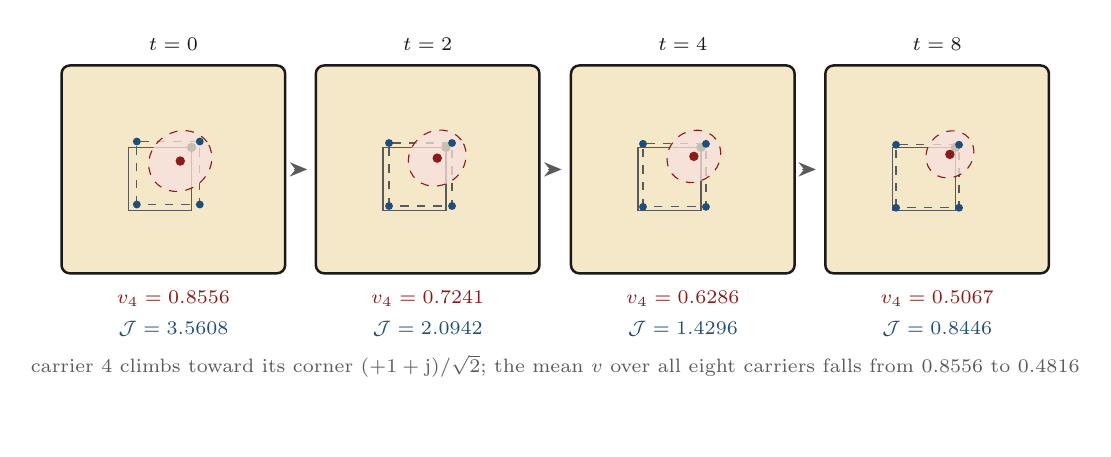
\begin{tikzpicture}[x=1cm,y=1cm]
    \path[use as bounding box] (-6.7,-2.75) rectangle (6.7,2.35);

    \foreach \xo/\tl/\ox/\oy/\px/\py/\ea/\eb/\ang/\vv/\jj in {
        -4.85/$t=0$/-0.1596/-0.1140/0.2203/0.2659/1.0409/0.9250/35.5/0.8556/3.5608,
        -1.62/$t=2$/-0.2267/-0.1619/0.3032/0.3586/0.9547/0.8519/37.0/0.7241/2.0942,
         1.62/$t=4$/-0.2641/-0.1886/0.3518/0.4144/0.8874/0.7942/38.3/0.6286/1.4296,
         4.85/$t=8$/-0.3042/-0.2173/0.4056/0.4775/0.7942/0.7137/40.2/0.5067/0.8446}{
      \begin{scope}[shift={(\xo,0.55)}]
        \draw[panel] (-1.42,-1.32) rectangle (1.42,1.32);
        \begin{scope}[scale=0.40]
          \draw[line width=0.5pt,color=inkgray]
            (-1.42,-1.30) rectangle (0.58,0.70);
          \fill[accentgreen] (0.58,0.70) circle (0.15);
          \begin{scope}[shift={(\ox,\oy)}]
            \draw[dashed,color=inkgray] (-1,-1) rectangle (1,1);
          \end{scope}
          \fill[redbg,opacity=0.75,rotate around={\ang:(\px,\py)}] (\px,\py) ellipse ({\ea} and {\eb});
          \draw[dashed,color=accentred,rotate around={\ang:(\px,\py)}] (\px,\py) ellipse ({\ea} and {\eb});
          \begin{scope}[shift={(\ox,\oy)}]
            \fill[accentblue] (1,1) circle (0.125);
            \fill[accentblue] (1,-1) circle (0.125);
            \fill[accentblue] (-1,1) circle (0.125);
            \fill[accentblue] (-1,-1) circle (0.125);
          \end{scope}
          \fill[accentred] (\px,\py) circle (0.15);
        \end{scope}
        \node[font=\scriptsize\bfseries,color=ink,anchor=south]
          at (0,1.38) {\tl};
        \node[font=\scriptsize,color=accentred,anchor=north] at (0,-1.42)
          {$v_4=\vv$};
        \node[font=\scriptsize,color=accentblue,anchor=north] at (0,-1.80)
          {$\mathcal J=\jj$};
      \end{scope}
    }
    \draw[grayarr] (-3.32,0.55) -- (-3.15,0.55);
    \draw[grayarr] (-0.09,0.55) -- (0.08,0.55);
    \draw[grayarr] (3.14,0.55) -- (3.31,0.55);

    \node[font=\scriptsize,color=inkgray] at (0,-1.95)
      {carrier 4 climbs toward its corner \((+1+\mathrm j)/\sqrt2\);
       the mean \(v\) over all eight carriers falls from
       \(0.8556\) to \(0.4816\)};
  \end{tikzpicture}
  \bottomnote{Each gradient step lowers the objective, and the signal likelihood rises as the objective falls.  Here the coefficients are held at their true values and plain gradient steps with a fixed step size move only \(\mathbf z\); the receiver instead solves \(\mathbf C\) conditionally and moves \(\mathbf z\) with Adam.}
\end{frame}

% =====================================================================
% 10. Receiver algorithms
% =====================================================================
\begin{frame}{Receiver algorithms}
  \centering
  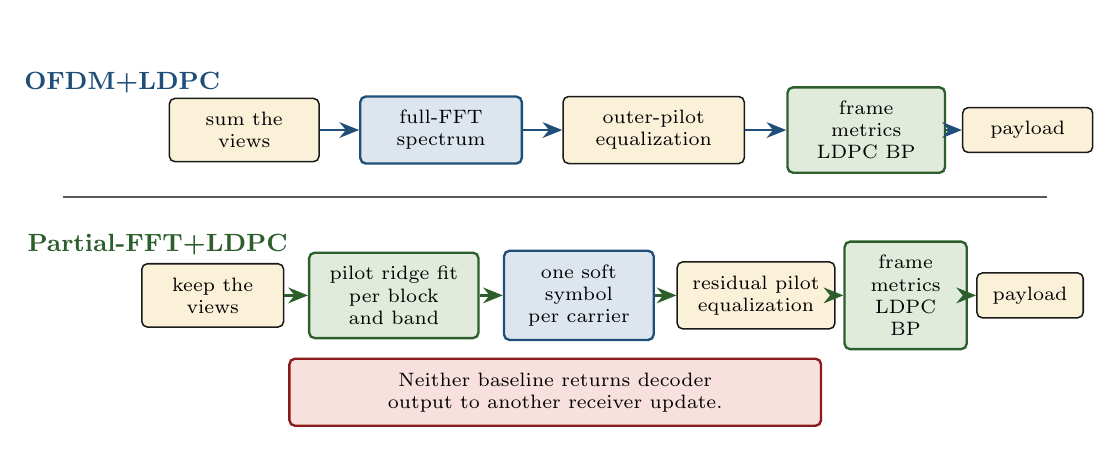
\begin{tikzpicture}[x=1cm,y=1cm]
    \path[use as bounding box] (-6.7,-2.75) rectangle (6.7,2.35);

    \node[font=\small\bfseries,color=accentblue] at (-5.50,1.65)
      {OFDM+LDPC};
    \node[card,text width=1.55cm,font=\scriptsize] (o1) at (-3.95,1.05)
      {sum the\\views};
    \node[bluecard,text width=1.70cm,font=\scriptsize] (o2) at (-1.45,1.05)
      {full-FFT\\spectrum};
    \node[card,text width=1.95cm,font=\scriptsize] (o3) at (1.25,1.05)
      {outer-pilot\\equalization};
    \node[goodcard,text width=1.65cm,font=\scriptsize] (o4) at (3.95,1.05)
      {frame metrics\\LDPC BP};
    \node[card,text width=1.30cm,font=\scriptsize] (o5) at (6.00,1.05)
      {payload};
    \draw[bluearr] (o1) -- (o2);
    \draw[bluearr] (o2) -- (o3);
    \draw[bluearr] (o3) -- (o4);
    \draw[bluearr] (o4) -- (o5);

    \draw[line width=0.6pt,color=inkgray] (-6.25,0.20) -- (6.25,0.20);

    \node[font=\small\bfseries,color=accentgreen] at (-5.05,-0.40)
      {Partial-FFT+LDPC};
    \node[card,text width=1.45cm,font=\scriptsize] (p1) at (-4.35,-1.05)
      {keep the\\views};
    \node[goodcard,text width=1.80cm,font=\scriptsize] (p2) at (-2.05,-1.05)
      {pilot ridge fit\\per block and band};
    \node[bluecard,text width=1.55cm,font=\scriptsize] (p3) at (0.30,-1.05)
      {one soft symbol\\per carrier};
    \node[card,text width=1.65cm,font=\scriptsize] (peq) at (2.55,-1.05)
      {residual pilot\\equalization};
    \node[goodcard,text width=1.20cm,font=\scriptsize] (p4) at (4.45,-1.05)
      {frame metrics\\LDPC BP};
    \node[card,text width=1.00cm,font=\scriptsize] (p5) at (6.03,-1.05)
      {payload};
    \draw[greenarr] (p1) -- (p2);
    \draw[greenarr] (p2) -- (p3);
    \draw[greenarr] (p3) -- (peq);
    \draw[greenarr] (peq) -- (p4);
    \draw[greenarr] (p4) -- (p5);

    \node[badcard,text width=6.40cm,font=\scriptsize] at (0,-2.28)
      {Neither baseline returns decoder output to another receiver update.};
  \end{tikzpicture}
\end{frame}

% =====================================================================
% 11. JUNA-Iterative
% =====================================================================
\begin{frame}{JUNA-Iterative}
  \centering
  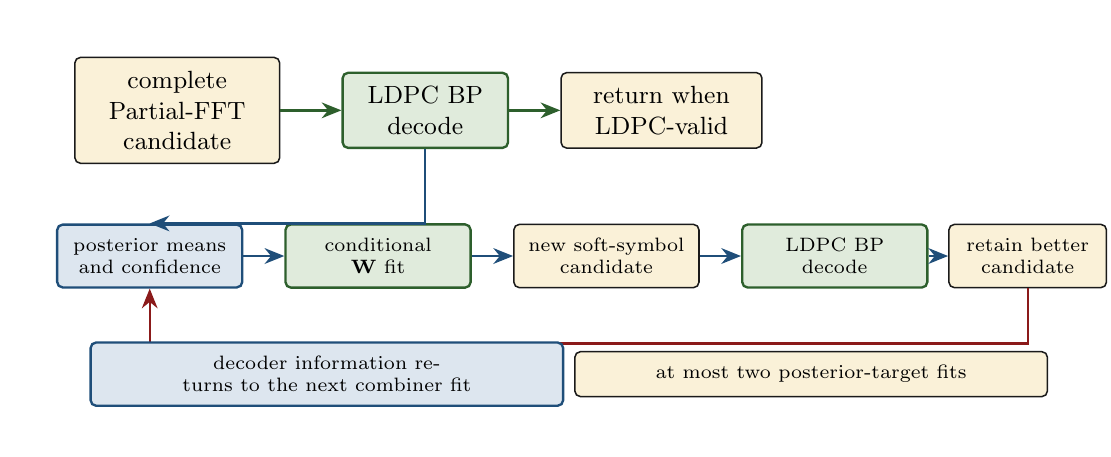
\begin{tikzpicture}[x=1cm,y=1cm]
    \path[use as bounding box] (-6.7,-2.75) rectangle (6.7,2.35);

    \node[card,text width=2.25cm] (start) at (-4.80,1.30)
      {complete Partial-FFT\\candidate};
    \node[goodcard,text width=1.75cm] (decode0) at (-1.65,1.30)
      {LDPC BP\\decode};
    \node[card,text width=2.20cm] (return) at (1.35,1.30)
      {return when\\LDPC-valid};
    \draw[greenarr] (start) -- (decode0);
    \draw[greenarr] (decode0) -- (return);

    \node[bluecard,text width=2.00cm,font=\scriptsize] (mean) at (-5.15,-0.55)
      {posterior means\\and confidence};
    \node[goodcard,text width=2.00cm,font=\scriptsize] (fit) at (-2.25,-0.55)
      {conditional\\\(\mathbf W\) fit};
    \node[card,text width=2.00cm,font=\scriptsize] (soft) at (0.65,-0.55)
      {new soft-symbol\\candidate};
    \node[goodcard,text width=2.00cm,font=\scriptsize] (decode) at (3.55,-0.55)
      {LDPC BP\\decode};
    \node[card,text width=1.65cm,font=\scriptsize] (best) at (6.00,-0.55)
      {retain better\\candidate};
    \draw[bluearr] (decode0.south) |- (mean.north);
    \draw[bluearr] (mean) -- (fit);
    \draw[bluearr] (fit) -- (soft);
    \draw[bluearr] (soft) -- (decode);
    \draw[bluearr] (decode) -- (best);
    \draw[redarr] (best.south) -- ++(0,-0.70) -| (mean.south);

    \node[bluecard,text width=5.65cm,font=\scriptsize] at (-2.90,-2.05)
      {decoder information returns to the next combiner fit};
    \node[card,text width=5.65cm,font=\scriptsize] at (3.25,-2.05)
      {at most two posterior-target fits};
  \end{tikzpicture}
  \bottomnote{Like turbo equalization, JUNA-Iterative repeats equalization and decoding.  It forms no \(\mathbf C\), has no free \(\mathbf z\), and never evaluates equation (30).}
\end{frame}

% =====================================================================
% 12. JUNA-(C,z)
% =====================================================================
\begin{frame}{JUNA-\(C,z\)}
  \centering
  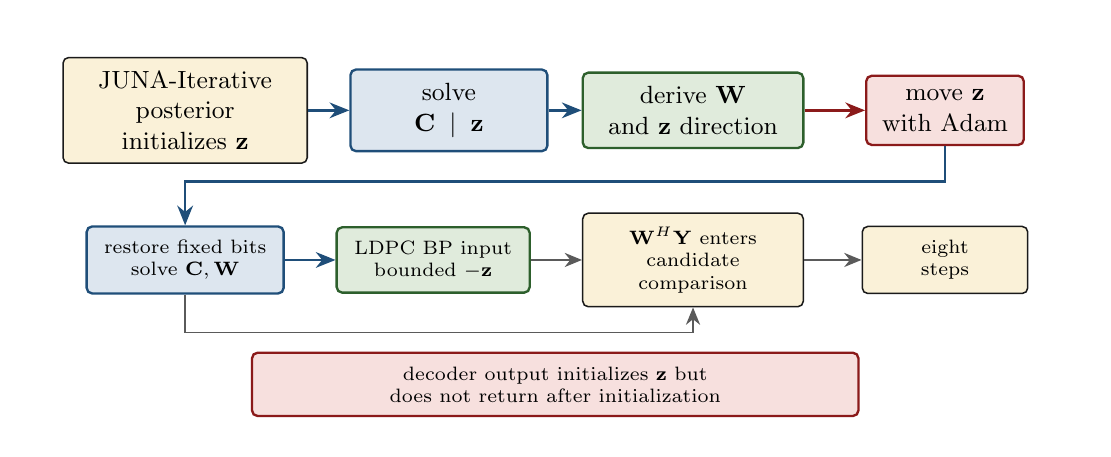
\begin{tikzpicture}[x=1cm,y=1cm]
    \path[use as bounding box] (-6.7,-2.75) rectangle (6.7,2.35);

    \node[card,text width=2.75cm] (initial) at (-4.70,1.30)
      {JUNA-Iterative posterior\\initializes \(\mathbf z\)};
    \node[bluecard,text width=2.15cm] (c) at (-1.35,1.30)
      {solve\\\(\mathbf C\mid\mathbf z\)};
    \node[goodcard,text width=2.45cm] (w) at (1.75,1.30)
      {derive \(\mathbf W\)\\and \(\mathbf z\) direction};
    \node[badcard,text width=1.65cm] (adam) at (4.95,1.30)
      {move \(\mathbf z\)\\with Adam};
    \draw[bluearr] (initial) -- (c);
    \draw[bluearr] (c) -- (w);
    \draw[redarr] (w) -- (adam);

    \node[bluecard,text width=2.15cm,font=\scriptsize] (again) at (-4.70,-0.60)
      {restore fixed bits\\solve \(\mathbf C,\mathbf W\)};
    \node[goodcard,text width=2.10cm,font=\scriptsize] (bp) at (-1.55,-0.60)
      {LDPC BP input\\bounded \(-\mathbf z\)};
    \node[card,text width=2.45cm,font=\scriptsize] (score) at (1.75,-0.60)
      {\(\mathbf W^H\mathbf Y\) enters\\candidate comparison};
    \node[card,text width=1.75cm,font=\scriptsize] (eight) at (4.95,-0.60)
      {eight\\steps};
    \draw[bluearr] (adam.south) -- ++(0,-0.45) -| (again.north);
    \draw[bluearr] (again) -- (bp);
    \draw[grayarr] (again.south) -- ++(0,-0.48) -| (score.south);
    \draw[grayarr] (bp) -- (score);
    \draw[grayarr] (score) -- (eight);

    \node[badcard,text width=7.35cm,font=\scriptsize] at (0,-2.18)
      {decoder output initializes \(\mathbf z\) but does not return after initialization};
  \end{tikzpicture}
  \bottomnote{JUNA-\(C,z\) conditionally solves the coefficients and moves only the relaxed bits.  Belief propagation receives \(-\mathbf z\), not \(\mathbf W^H\mathbf Y\).}
\end{frame}

% =====================================================================
% 13. JUNA-Direct-(C,z)
% =====================================================================
\begin{frame}{JUNA-Direct-\(C,z\)}
  \centering
  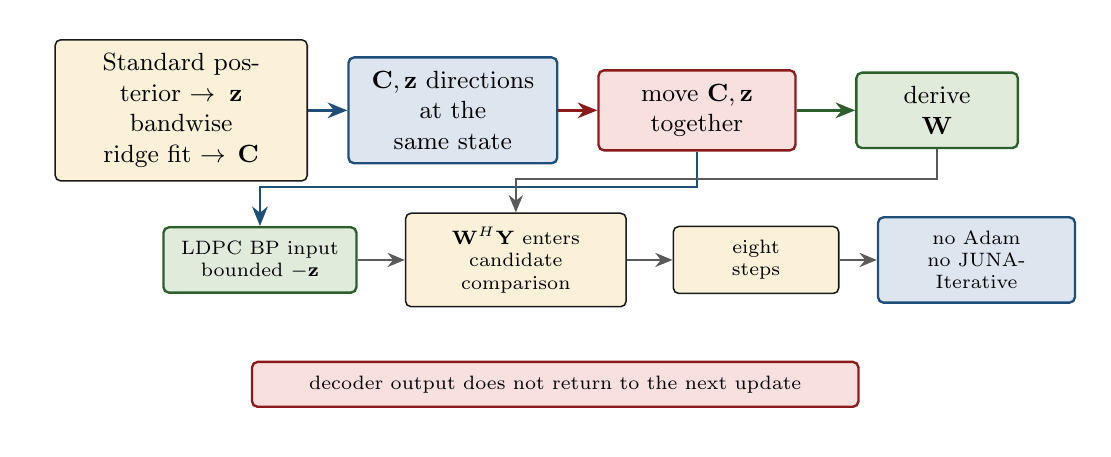
\begin{tikzpicture}[x=1cm,y=1cm]
    \path[use as bounding box] (-6.7,-2.75) rectangle (6.7,2.35);

    \node[card,text width=2.85cm] (initial) at (-4.75,1.30)
      {Standard posterior \(\to\mathbf z\)\\bandwise ridge fit \(\to\mathbf C\)};
    \node[bluecard,text width=2.30cm] (dir) at (-1.30,1.30)
      {\(\mathbf C,\mathbf z\) directions\\at the same state};
    \node[badcard,text width=2.15cm] (move) at (1.80,1.30)
      {move \(\mathbf C,\mathbf z\)\\together};
    \node[goodcard,text width=1.70cm] (w) at (4.85,1.30)
      {derive\\\(\mathbf W\)};
    \draw[bluearr] (initial) -- (dir);
    \draw[redarr] (dir) -- (move);
    \draw[greenarr] (move) -- (w);

    \node[goodcard,text width=2.10cm,font=\scriptsize] (bp) at (-3.75,-0.60)
      {LDPC BP input\\bounded \(-\mathbf z\)};
    \node[card,text width=2.45cm,font=\scriptsize] (score) at (-0.50,-0.60)
      {\(\mathbf W^H\mathbf Y\) enters\\candidate comparison};
    \node[card,text width=1.75cm,font=\scriptsize] (eight) at (2.55,-0.60)
      {eight\\steps};
    \node[bluecard,text width=2.15cm,font=\scriptsize] (none) at (5.35,-0.60)
      {no Adam\\no JUNA-Iterative};
    \draw[bluearr] (move.south) -- ++(0,-0.45) -| (bp.north);
    \draw[grayarr] (w.south) -- ++(0,-0.38) -| (score.north);
    \draw[grayarr] (bp) -- (score);
    \draw[grayarr] (score) -- (eight);
    \draw[grayarr] (eight) -- (none);

    \node[badcard,text width=7.35cm,font=\scriptsize] at (0,-2.18)
      {decoder output does not return to the next update};
  \end{tikzpicture}
  \bottomnote{JUNA-Direct-\(C,z\) moves the coefficient and relaxed-bit variables together.  The weights are derived from the updated coefficients and remain outside equation (30).}
\end{frame}

% =====================================================================
% 14. Takeaway
% =====================================================================
\begin{frame}[plain]
  \centering
  \vspace{0.22cm}
  {\bfseries\LARGE Takeaway\par}
  \vspace{0.18cm}
  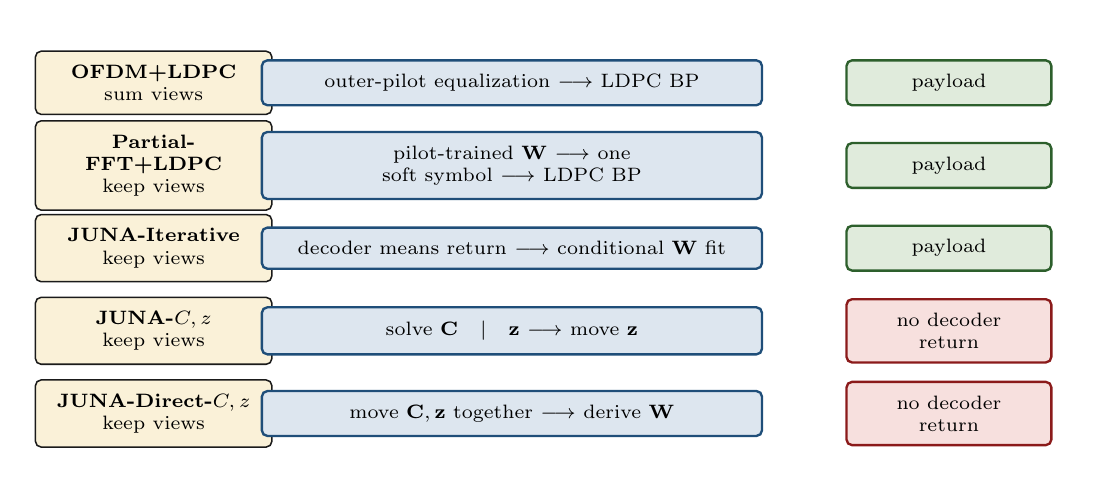
\begin{tikzpicture}[x=1cm,y=1cm]
    \path[use as bounding box] (-6.7,-3.00) rectangle (6.7,2.55);

    \node[card,text width=2.65cm,font=\scriptsize] at (-5.10,1.85)
      {\textbf{OFDM+LDPC}\\sum views};
    \node[bluecard,text width=6.00cm,font=\scriptsize] at (-0.55,1.85)
      {outer-pilot equalization \(\longrightarrow\) LDPC BP};
    \node[goodcard,text width=2.25cm,font=\scriptsize] at (5.00,1.85)
      {payload};

    \node[card,text width=2.65cm,font=\scriptsize] at (-5.10,0.80)
      {\textbf{Partial-FFT+LDPC}\\keep views};
    \node[bluecard,text width=6.00cm,font=\scriptsize] at (-0.55,0.80)
      {pilot-trained \(\mathbf W\) \(\longrightarrow\) one soft symbol
       \(\longrightarrow\) LDPC BP};
    \node[goodcard,text width=2.25cm,font=\scriptsize] at (5.00,0.80)
      {payload};

    \node[card,text width=2.65cm,font=\scriptsize] at (-5.10,-0.25)
      {\textbf{JUNA-Iterative}\\keep views};
    \node[bluecard,text width=6.00cm,font=\scriptsize] at (-0.55,-0.25)
      {decoder means return \(\longrightarrow\) conditional \(\mathbf W\) fit};
    \node[goodcard,text width=2.25cm,font=\scriptsize] at (5.00,-0.25)
      {payload};

    \node[card,text width=2.65cm,font=\scriptsize] at (-5.10,-1.30)
      {\textbf{JUNA-\(C,z\)}\\keep views};
    \node[bluecard,text width=6.00cm,font=\scriptsize] at (-0.55,-1.30)
      {solve \(\mathbf C\mid\mathbf z\) \(\longrightarrow\) move \(\mathbf z\)};
    \node[badcard,text width=2.25cm,font=\scriptsize] at (5.00,-1.30)
      {no decoder\\return};

    \node[card,text width=2.65cm,font=\scriptsize] at (-5.10,-2.35)
      {\textbf{JUNA-Direct-\(C,z\)}\\keep views};
    \node[bluecard,text width=6.00cm,font=\scriptsize] at (-0.55,-2.35)
      {move \(\mathbf C,\mathbf z\) together \(\longrightarrow\) derive \(\mathbf W\)};
    \node[badcard,text width=2.25cm,font=\scriptsize] at (5.00,-2.35)
      {no decoder\\return};
  \end{tikzpicture}
  \vspace{0.08cm}

  {\small Pilots constrain \(\mathbf C\); parity checks constrain
   \(\mathbf z\); equation (30) scores the coefficient-and-bit pair in the
   received views.\par}
  \vspace{0.12cm}
  {\itshape\small Only JUNA-Iterative returns decoder information to the next update.\par}
\end{frame}

% =====================================================================
% 15. Posterior-variance alternative
% =====================================================================
\begin{frame}{Posterior variance}
  \centering
  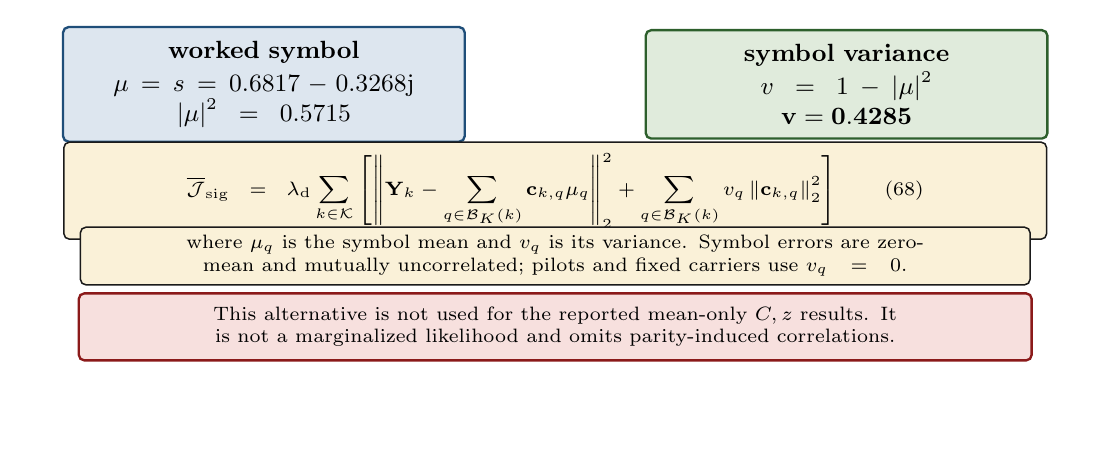
\begin{tikzpicture}[x=1cm,y=1cm]
    \path[use as bounding box] (-6.7,-2.78) rectangle (6.7,2.42);

    \node[bluecard,text width=4.75cm] at (-3.70,1.70)
      {\textbf{worked symbol}\\[0.10em]
       \(\mu=s=0.6817-0.3268\mathrm j\)\\
       \(\left|\mu\right|^2=0.5715\)};
    \node[goodcard,text width=4.75cm] at (3.70,1.70)
      {\textbf{symbol variance}\\[0.10em]
       \(v=1-\left|\mu\right|^2\)\\
       \(\mathbf{v=0.4285}\)};

    \node[card,text width=12.20cm,inner sep=4pt] at (0,0.35)
      {\scriptsize
       \(\displaystyle
       \overline{\mathcal J}_{\mathrm{sig}}
       =\lambda_{\mathrm d}\sum_{k\in\Kset}
       \left[
       \left\|\mathbf Y_k-
       \sum_{q\in\Bset_K(k)}\mathbf c_{k,q}\mu_q\right\|_2^2
       +\sum_{q\in\Bset_K(k)}
       v_q\norm{\mathbf c_{k,q}}_2^2
       \right]\qquad\text{(68)}\)};
    \node[card,font=\scriptsize,text width=11.85cm,align=center,inner sep=3pt]
      at (0,-0.48)
      {where \(\mu_q\) is the symbol mean and \(v_q\) is its variance.
       Symbol errors are zero-mean and mutually uncorrelated; pilots and
       fixed carriers use \(v_q=0\).};

    \node[badcard,text width=11.75cm,font=\scriptsize] at (0,-1.38)
      {This alternative is not used for the reported mean-only \(C,z\)
       results.  It is not a marginalized likelihood and omits
       parity-induced correlations.};
  \end{tikzpicture}
  \bottomnote{Equation (68) replaces only the signal term of equation (30).}
\end{frame}

\end{document}
